\chapter{REVIEW OF RELATED LITERATURE}

Now that you have established what your study is, this section provides you the ability to look into your research area in order to find out what is the state-of-the-art regarding your topic of interest. By the end of this section, you should already have an idea of what has been done in relation to your work, what findings they had about their studies, and how your own study factors into what was observed (e.g. improvements based upon the studies’ recommendations, techniques that can be borrowed, delineating where previous work ends and where your study begins).

This is an equation:
\[
    x = \frac{-b \pm \sqrt{b^2 - 4ac}}{2a}
\]

Although it discusses a variety of literature, it is still important to maintain a general flow within your discussion. Make use of transitions and other literary means to connect the ideas of each discussed article. One way to do this is to first organize your articles into general topics of discussion. You may then introduce the flow of these topics in the first few paragraphs of this section, and use the topic outline you created as your guide in delivering, comparing and contrasting what ideas you may wish to present about the literature. You can also use the themes as your sub headings. Finally, summarize your literature review by briefly going through the key ideas of previous work, identify points for improvement, and state what your study can do to contribute in addressing those points.

Last but not the least, do not forget to put proper citations to the ideas you will present. More often than not, whatever idea you state here came from another source, so ensure that you acknowledge the article/book/other reference you may have lifted it from.
In order to guide you in writing, as well as to summarize the points mentioned above, here are some questions that may help your structure your discussion:

\begin{enumerate}
\item What previous works are closely connected with your own study? Who initiated these studies?
\item What objectives did these studies have? If they presented any research questions, what were these and how similar or different are they from your own set of questions?
Describe the methods used in these studies.
If there are test subjects, what is the general profile of their subjects?
\item What instruments did they use to acquire and measure their data?
\item What were the findings gathered from the studies? 
\item What issues, if any (e.g. flaws or gaps in the methodology), were encountered during the implementation of the study? In what way did the researchers attempt to address these issues? Were they successful in resolving these issues? Why or why not?
\item What conclusions did these studies have? What recommendations did they present, and which of these recommendations may be addressed through your study?
\item What other improvements could be done that was not mentioned in the study? How will your study incorporate these improvements?
\item In what way is your study different or novel given these previous studies? Where do their studies end, and where will yours begin?
\end{enumerate}

Below is a sample entry from a literature review. You may use this as basis for your own work.

\section{Motivation and ECAs}
In applying motivational concepts to ECAs, some previous work includes studies by Rebolledo-Mendez et al. [9] and Graesser et al [4, 5].
Rebolledo-Mendez et al. [9] investigated the effect of a motivational version of Ecolab, an ITS for teaching primary school children the topic of Ecology, particularly about food chains and food webs. In implementing the motivational extension, they modeled three motivational traits identified as key in the learning context. These are effort, confidence, and independence from the tutor [9]. The motivational on-screen character, which they named as Paul, was designed to provide feedback before and after each activity. Each post-activity feedback was based on the motivational model of the learner, and using this, Paul encourages the learner: to exert more effort, to be more independent, or to become more confident [9].

%\begin{figure}[h] 
%    \centering
%    
\includegraphics[width=0.6\textwidth,height=0.2\textheight]{figures/Figure_2-1.png}
%    \caption{Expressions of Paul of M-Ecolab [10].}
%    \label{fig:Figure_2-1.png}
%\end{figure}

 The results of the study showed that through modeling motivation and adjusting motivational reaction, the de-motivated, low, and average students were able to significantly increase their post-test scores. It also, however, showed that highly motivated and high ability students had no increase in test scores. The researchers noted that this could be due to the “ceiling effect”. Nevertheless, it was highlighted that the effects on learning by these motivating techniques were different, depending on the students’ ability and motivation. An example would be adjusting spoken feedback considering the learners’ motivational state as an important influence at post-activity time [9].
There were, however, some limitations to the study. One of these was that the results were derived from a very small sample. Another limitation they indicated was that adapting feedback and character’s reactions, in conjunction with a quiz, constitute only a first step in the study of motivating techniques in ITSs; thus, general guidelines could be used in order to improve student motivation [9].
On the other hand, Graesser et al. [4] developed a computer tutor called AutoTutor, which simulated the discourse patterns and pedagogical strategies of a typical human tutor. It was designed for college students in introductory computer literacy courses, who learn the fundamentals of hardware, operating systems, and the Internet [4].

\begin{figure}[!ht] 
    \centering
    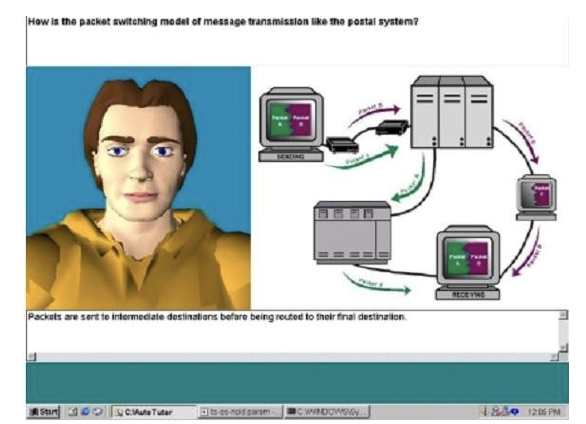
\includegraphics[width=0.6\textwidth,height=0.3\textheight]{figures/Figure_2-2.png}
    \caption{The AutoTutor Interface.}
    \label{fig:Figure_2-2.png}
\end{figure}

AutoTutor works by initiating a conversation with the student. It appears as a talking head that acts as a dialogue partner with the learner, who contributes to the conversation via input from the keyboard. One thing notable about the tutor is that it encourages the learner to articulate answers that are lengthy and require deep reasoning – examples of which include answers to why, how, and what-if questions. There is a multi-turn dialogue involved between AutoTutor and the student, encouraging the student to construct the knowledge and discover what he or she has mastered, rather than bombarding the student with the information to master [4].
Results of the study show that this strategy of AutoTutor was able to influence learning and mastery of students. Comparing students who used AutoTutor to those who only reread the topic and to the control group who did not reread, AutoTutor was able to help students answer more questions which were used in an actual computer literacy course, garnering a greater score than the two other groups [4]. 
In terms of the conversational smoothness and pedagogical quality of dialogue, an experiment was done where students were asked to point out which dialogue moves were generated by human tutors and which ones were by AutoTutor. Results show that the students were unable to discriminate the dialogue moves that were computer-generated compared to those from human tutors. In reality, half of the dialogue was by human tutors and the other half by AutoTutor. This proved the ability of AutoTutor to accurately simulate a human tutor [4].
In a related study, Graesser et al. [5] was able to determine that during interactions with the AutoTutor, confusion was a great predictor of post-test scores. The study showed that when the learner is confused the learner experiences cognitive disequilibrium and thinking. It is presumed that the other frequent emotions such as frustration, bored and flow play a more prominent role in other learning environments and population of learners. It is therefore suggested that further research be conducted on these frequent emotions to discover different strategies and dialogues that will promote both learning gains and more engagement for the students [5].


\section {New Sample Subsection}
This is added in between existing subsections.

\section{Sample Subsection}
Blah blah blah blah!

\section{Sample Sample Subsection New}
This is added after the last existing subsection. Updated the TOC, it works.
